\documentclass[a4paper, 12pt]{scrartcl}
 \usepackage{fullpage}
 \usepackage[ngerman]{babel}
 \usepackage[utf8]{inputenc}
 \usepackage{hyperref}
 \usepackage{amsmath}
 \usepackage{graphicx}
 \usepackage{color}


\title{T8 Brownsche Molekularbewegung}

% Nice san serif font
\renewcommand{\familydefault}{\sfdefault}

\newcommand{\mean}[1]{\left< #1 \right>}

\hyphenation{rest-lichen}


\begin{document}
\let\endtitlepage\relax
\begin{titlepage}

\begin{minipage}{0.5\textwidth}
\begin{flushleft}
\makeatletter
Universität Potsdam\\
Institut für Physik und Astronomie\\
Grundpraktikum
\makeatother
\end{flushleft}
\end{minipage}%
%
\begin{minipage}{0.5\textwidth}
\begin{flushright}
\makeatletter
\textbf{\the\month/\the\year}
\makeatother
\end{flushright}
\end{minipage}

\begin{center}
\makeatletter
\Large \textbf{\@title}
\end{center}
\makeatother
\end{titlepage}

\section*{Ziel des Versuches}

Die Brownsche Bewegung wurde 1826 von R. Brown entdeckt, konnte aber erst 1905 durch Einstein erklärt werden.\\
Sie werden die Brownsche Bewegung eines Polystyrolpartikels in Wasser unter dem Mikroskop beobachten. Die Brownsche Bewegung beschreibt die ``Zitterbewegung'' eines Teilchens als Resultat der Stöße der umgebenden Flüssigskeitsmoleküle. Sie werden  die Ortsveränderungen eines Partikels anhand einer Bildsequenz mit einem Mikroskop bestimmen und aus diesen die Diffusionskonstante, die Boltzmann-Konstante und die Avogadro-Konstante berechnen.


\section*{Hinweise zur Vorbereitung}
Lesen Sie den theoretischen Hintergrund und die Literatur. Beantworten Sie die folgenden Fragen.

\begin{itemize}
  \item Wie groß ist ein Wassermolekül und wie viele Größenordnungen liegen zwischen ihm und einem Polystyrolpartikel mit einem Radius von $1 \mu$m?
  \item Wie bewegen sich zwei kugelförmige Körper nach einem Stoß, wenn ihre Massen sehr unterschiedlich sind und der schwere Körper ruht?
  \item Was ist eine Normalverteilung/Gaußverteilung? Was beschreiben ihr Mittelwert und ihre Standardabweichung?
  \item Was bedeuten die Größen in der Einstein-Smoluchowski-Gleichung (\ref{eq:einstein}) und wie kann die Gleichung verstanden werden?
  \item Was bedeuten die Größen in der Gleichung für die Diffusionskonstante (\ref{eq:diff}) und wie kann die Gleichung verstanden werden?
  \item Was besagt das Ergodentheorem? Wie kann es überprüft werden?
\end{itemize}

\section*{Theoretischer Hintergrund}

Die \textbf{Brownsche Bewegung} beschreibt die zufällige Bewegung eines kleinen Körpers in einer Flüssigkeit. Sie entsteht durch die thermische Bewegung der umgebenden Flüssigkeitsmoleküle, die gegen den Körper stoßen.
Thermische Bewegung ist ein Ausdruck der thermischen Energie, also der Energie, die Teilchen aufgrund ihrer Temperatur aufweisen.\\
Eine höhere Temperatur führt zu einer höheren Geschwindigkeit der Moleküle. Wird die Temperatur jedoch reduziert, dann verringert sich auch die Geschwindigkeit der Moleküle, bis sie schließlich ruhen. Die Temperatur, bei der alle Moleküle ruhen, ist der absolute Nullpunkt und entspricht $0 \,$K.\\

Da die Brownsche Bewegung zufällig ist, können keine präzisen Voraussagen über sie gemacht werden, aber mithilfe der Statistik lassen sich trotzdem allgemeine Aussagen über sie formulieren.\\
Die wichtigsten Mittel in der Statistik sind der Mittelwert und die Standardabweichung. Der \textbf{Mittelwert} $\mean{\Delta x}$ gibt die durchschnittliche Verschiebung in x-Richtung an und die \textbf{Standardabweichung} $\sigma$ gibt die durchschnittliche Verschiebung von $\mean{\Delta x}$ an. Für diskrete Prozesse sind sie folgendermaßen definiert:
\begin{align}
  \mean{x} & = \frac{1}{N} \sum_{i=1}^{N} x_i, \\
  \sigma & = \sqrt{\mean{ {\left( x - \mean{x} \right)}^2 }} = \sqrt{\frac{1}{N - 1} \sum_{i=1}^{N} {\left( x_i - \mean{x} \right)}^2}.
\end{align}
Um Prozesse genauer zu beschreiben werden Wahrscheinlichkeitsverteilungen verwendet. Sie geben an, mit welcher Wahrscheinlichkeit ein Wert gemessen wird. Histogramme dienen dazu, solch eine Verteilung mit endlich vielen Messwerten zu beschreiben.\\
Die Verteilung, die hier von Bedeutung ist, ist die Normalverteilung. Sie ist durch die Verteilungsfunktion
\begin{equation}
  f(\Delta x, \mean{\Delta x}, \sigma) = \frac{1}{\sqrt{2 \pi \sigma^2}} e^{- \frac{(\Delta x - \mean{\Delta x})^2}{2 \sigma^2}} \label{eq:gauss}
\end{equation}
definiert. Der Mittelwert der Normalverteilung ist ihr Maximum und die Standardabweichung gibt ihre Breite an. Eine Normalverteilung ist in der Abbildung \ref{fig:histo} dargestellt.\\

\begin{figure}[h!]
  \centering
  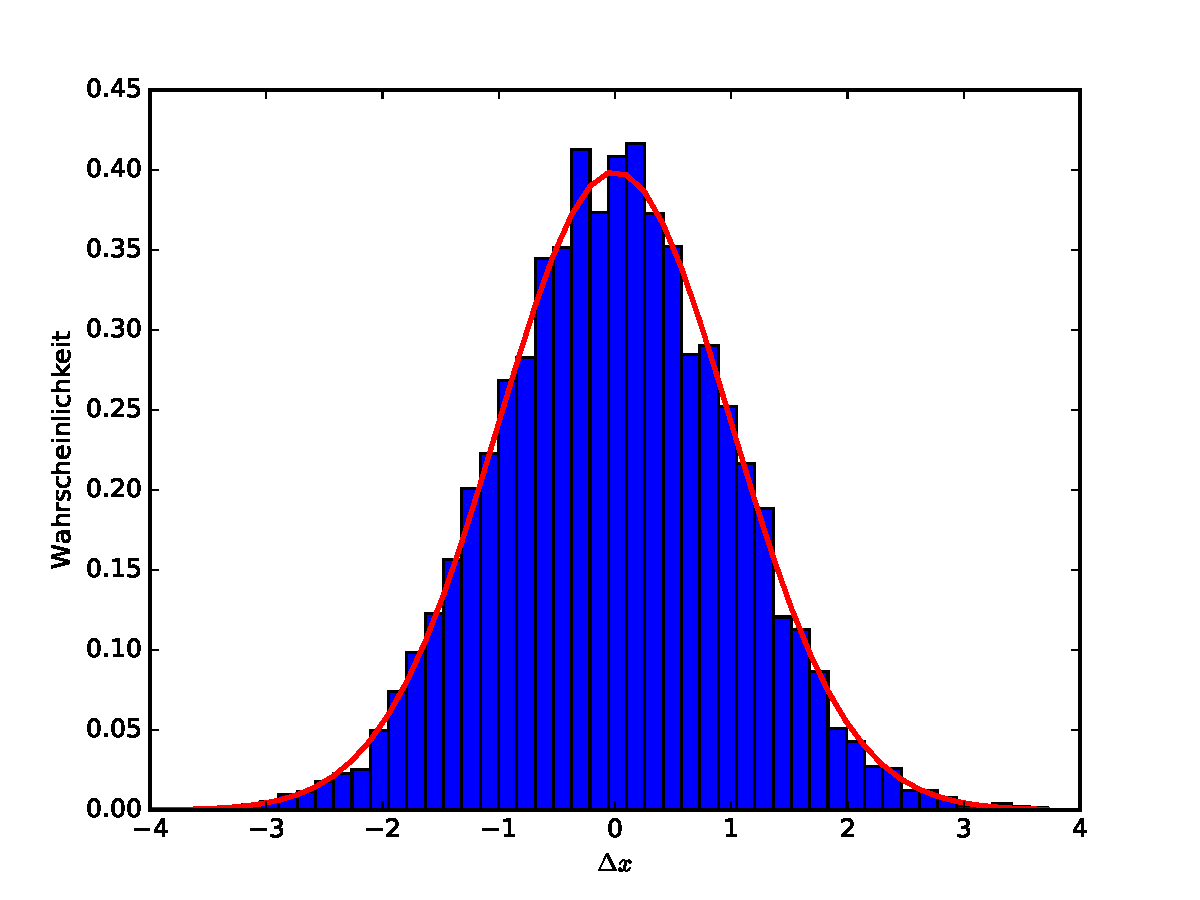
\includegraphics[width=0.7\textwidth]{figures/histogram}
  \caption{Histogram und zugehörige Normalverteilung}\label{fig:histo}
\end{figure}
Um diese Hilfsmittel effizient auf die Brownsche Bewegung anwenden zu können, muss sie noch formal beschrieben werden. Dazu eignet sich das Model eines \textbf{random walks}. Ein \emph{random walk} in einer Dimension funktioniert folgendermaßen: In regelmäßigen Zeitabständen $\tau$ wird eine Münze geworfen. Zeigt sie Kopf bewegt sich das Teilchen einen Schritt nach rechts und zeigt sie Zahl einen Schritt nach links. Die Schrittweite $\delta$ ist für beide Fälle gleich groß. Um die Bewegung zu charakterisieren kann die Diffusionskonstante $D$ definiert werden
\begin{equation}
  D = \frac{\delta^2}{2 \tau}. \label{eq:diff_random}
\end{equation}
Sie gibt an, wie weit sich das Teilchen durch die zufällige Bewegung im Mittel, nach einem Schritt, von der Nulllage entfernen kann.\\
Es ist intuitiv klar, dass sich das Teilchen im Durchschnitt nicht von seiner Ursprungslage wegbewegt, ist der Ursprung bei $\Delta x = 0$, dann ist also $\mean{\Delta x} = 0$. Aber was ist mit der Standardabweichung? Da hier $\Delta x^2$ eine Rolle spielt, löschen sich die Schritte nach links und rechts nicht gegenseitig aus.
Desto größer die Schrittweite ist, desto weiter wird sich das Teilchen im Durchschnitt von der Nulllage entfernen. Alternativ kann auch die Zeit zwischen zwei Schritten verringert werden. Aus dieser Überlegung ergibt sich die Diffusionskonstante $D$ für den Versuch, denn die Diffusionskonstante aus (\ref{eq:diff_random}) beschreibt nur den \emph{random-walk}.\\
Um sie benutzen zu können, müsste die durchschnittliche Zeit zwischen den Stößen und die durchschnittliche Verschiebung nach einem Stoß bekannt sein. Diese Größen können aber nicht experimentell ermittelt werden. Stattdessen kann die Verschiebung zwischen zwei Messungen als \emph{random-walk} aufgefasst werden. Die Schrittweite dieses \emph{random-walks} ist nicht konstant, aber wenn die Bewegung genügend lange beobachtet wird, kann die mittlere Verschiebung als Schrittweite $\delta$ gewählt werden. Das ist aber gerade die Standardabweichung $\sigma$ der Verschiebung $\Delta x$. Und die Zeit zwischen zwei Schritten ist die Zeit zwischen zwei Messungen $t$. Damit ist die experimentell ermittelte Diffusionskonstante
\begin{equation}
  D = \frac{\sigma^2}{2 t}. \label{eq:diff}
\end{equation}
Sie gibt an, wie weit sich das Teilchen in einer Zeit $t$ im Durchschnitt von seinem Ursprung entfernt.\\

Wird der \emph{random walk} nur eine kurze Zeit beobachtet, können aufgrund der zufälligen Natur keine genauen Aussagen gemacht werden. Erst für lange Zeitreihen werden sich die Messwerte an die theoretischen Werte annähern. Alternativ können aber auch viele \emph{random walks} für kurze Zeit betrachtet werden. Das ist das \textbf{Ergodentheorem}. Es besagt, dass es für zufällige thermodynamische System äquivalent ist, ein System über lange Zeit zu mitteln, oder viele Systeme über kurze Zeit. In dem Experiment wird eine lange Brownsche Molekularbewegung beobachtet, zur Auswertung muss sie aber in viele kleine Abschnitte zerlegt werden. Das Ergodentheorem ermöglicht es die lange Bewegung mit den vielen kleinen gleich zu setzen.\\
Bei einem \emph{random walk} in zwei Dimensionen, wie er in dem Versuch gemessen wird, können die beiden Richtungen unabhängig voneinander, als zwei \emph{random walks}, betrachtet werden. Es werden also gleichzeitig zwei Münzen geworfen, eine für die Bewegung nach links und rechts und eine für die Bewegung nach oben und unten.\\


Damit kann die Brownsche Bewegung beschrieben werden. Es fehlt aber noch der Zusammenhang zwischen ihr und der thermischen Energie der Flüssigkeit. Die thermische Energie der umgebenden Flüssigkeitsmoleküle führt zu der Bewegung, dass heißt, die thermische Energie der Flüssigkeit ist gleich der Bewegungsenergie. Diese setzt sich zusammen aus der Diffusion und der Reibung des Teilchens in der Flüssigkeit. Die entstehende Gleichung heißt die  \textbf{Einstein-Smoluchowski} Gleichung.
\begin{equation}
  D C = k_B T \label{eq:einstein}
\end{equation}
Dabei ist $k_B$ die Boltzmann-Konstante, $T$ die Temperatur in K und $C$ die Stokessche Reibungskonstante. Die Reibungskonstante gibt an, wie stark die Reibung auf eine Kugel mit Radius $r$ in einer Flüssigkeit mit Viskosität $\eta$ wirkt.
\begin{equation}
  C = 6 \pi \eta r
\end{equation}
In der Einstein-Smoluchowksi Gleichung taucht wieder die Diffusionskonstante auf. Allerdings wird bei der Herleitung in Gleichung (\ref{eq:einstein}) nicht direkt von einem \emph{random walk} ausgegangen. Das $D$ kommt hier von der Diffusionsgleichung
\begin{equation}
  \frac{\partial c}{\partial t}(x, t) = D \frac{\partial^2 c}{\partial x^2} (x, t). \label{eq:diffusion}
\end{equation}
Diese Gleichung beschreibt die zeitliche Änderung der Konzentration $c$, abhängig von ihrer räumlichen Verteilung. Eine konstante Lösung der Diffusion ist es, dass sich die Konzentration solange ändert, bis sie überall gleich ist. Die Geschwindigkeit dieser Änderung ist durch die Diffusionskonstante gegeben.\\
Es lässt sich zeigen, dass die Diffusionskonstante des \emph{random walks} genau der Diffusionskonstante der Thermodynamik entspricht, was auf die enge Verbindung zwischen dem \emph{random walk} und der Brownschen Bewegung hindeutet [\ref{it:bergmann}].

\section*{Durchführung}

\subsection*{Teil 1 - Simulation}

Es steht eine Simulation zur Verfügung, bei der drei Parameter verändert werden können, die Anzahl der Teilchen, die Zeitspanne und die Anzahl der Stöße pro Sekunde. Für die Statistik ist die Veränderung der Zeit und der Anzahl der Stöße äquivalent: Anstatt die Simulation $10$ Sekunden mit $30\times1$ Stößen laufen zu lassen, können auch $30\times10$ Stöße pro Sekunde für $1$ Sekunde durchgeführt werden. Nach einem Lauf wird ein Diagramm dargestellt, in dem die Schrittweite gegen eine Normalverteilung aufgetragen ist.\\
\begin{enumerate}

    \item Die Unterschiede der gemessenen Verteilung und der Normalverteilung sollen für drei verschiedene Messreihen verglichen werden. Jede Simulation sollte mehrmals durchgeführt werden, da die Qualität der Ergebnisse teilweise stark schwankt.

    \begin{enumerate}

      \item Eine kurze Messreihe mit wenigen Teilchen. (z.B. $1$ Teilchen über $5$ Sekunden und $30\times10$ Stöße)

      \item Eine lange Messreihe mit wenigen Teilchen. (z.B. $1$ Teilchen über $5$ Sekunden und $30\times100$ Stöße; entspricht $1$ Teilchen über $50$ Sekunden und $30\times10$ Stöße)

      \item Eine kurze Messreihe mit vielen Teilchen. (z.B. $10$ Teilchen über $5$ Sekunden und $30\times10$ Stöße)

    \end{enumerate}

\end{enumerate}


\subsection*{Teil 2 - Experiment}

Abgesehen von der Suche nach dem Objektmikrometer sollte die ganze Zeit mit der maximalen Vergrößerung gearbeitet werden. Außerdem sollte die Lichtquelle so eingestellt sein, dass das Bild nicht überbelichtet wird. \\
Zur Beobachtung wird das Programm \emph{Grab \& Measure} verwendet. Um das Live-Video zu aktivieren, muss der Button \emph{Live} auf der rechten Schaltleiste angeklickt werden.

\begin{enumerate}

  \item Zuerst muss das Objektmikrometer fotografiert werden. Dazu muss das Objektmikrometer mit der Skala nach oben auf den Objekttisch gelegt und fokussiert werden. Anschließend wird mithilfe der Software und der Funktion \emph{Grab} ein Foto von $5$ Skalenstrichen gemacht.

  \item Um die Skalierung der Abstände in den Bilder zu bestimmen, muss das Objektmirometer vermessen werden. Dazu wird das Bild durch Doppelklick in der linken Schaltfläche ausgewählt. In dem Bild wird mit einem Linksklick ein Messpunkt am äußersten linken Strich platziert. Dieser Messpunkt kann mit einem Rechtsklick \emph{Punktkoordinaten speichern} gespeichert werden. Danach muss ein zweiter Messpunkt am äußersten rechten Strich gesetzt und gespeichert werden. Beide Punkten sollten auf einer horizontalen Linie liegen. Zur Hilfe kann das Fadenkreuz mittels des \emph{Fadenkreuz-Buttons} auf der rechten Schaltleiste eingeblendet werden. Der Abstand zwischen zwei Skalenstrichen beträgt $10 \, \mu$m.


  \item Jetzt kann das Präparat angefertigt werden. Dazu wird ein Tropfen der Polystyrol-Lösung auf einen Objektträger gegeben. Links und rechts neben den Tropfen werden Deckplättchen gelegt und auf diese beiden ein weiteres, sodass der Tropfen flach gedrückt wird. Vorsicht: Ist der Tropfen zu klein, berührt er das obere Deckplättchen nicht und es kann nicht mikroskopiert werden. Ist der Tropfen aber zu groß, berührt er die äußeren Deckplättchen und es entstehen Strömungen, die die Messergebnisse verfälschen.

  \item Nachdem das Präparat angefertigt wurde, kann mikroskopiert werden. Dazu wird der Objekttisch etwas heruntergefahren und das Präparat gegen das Objektmikrometer ausgetauscht. Danach kann der Objekttisch wieder langsam hochgefahren werden. Dabei zeigen sich verschiedene Schichten. Zuerst wird eine zerkratze Schicht sichtbar, dass ist die Oberseite des Deckplättchens, danach kommt eine zerkratzte Schicht mit ruhenden schwarzen Kügelchen, dass ist die Unterseite des Plättchens. Ab hier muss der Tisch noch ein kleines Stück nach oben gefahren werden, dann sollten die Polystyrol-Partikel als kleine, zitternde schwarze Kügelchen zu sehen sein.

  \item Jetzt kann eine Messreihe aufgenommen werden. Dazu muss ein einzelnes Polystyrol-Kügelchen gefunden und in der Mitte des Bildschirms zentriert werden. In der Nähe sollte auch kein Schmutz sein, sodass die Brownsche Bewegung ungestört beobachtet werden kann. Während der Messung darf an dem Mikroskop nicht verstellt werden und es sollte möglichst auch nicht am Tisch gewackelt werden.\\
  Nach einem Klick auf das \emph{Disketten}-Symbol in der rechten Leiste und der Einstellung des Zeitintervall  auf $2 \,$s, kann die Aufnahme durch einen Mausklick auf den \emph{Start}-Button gestartet werden.\\
  Die Messreihe besteht aus $101$ Bildern, vermutlich wird sich das Kügelchen währenddessen aus dem Bild bewegen. Sollte die Messreihe aus weniger als $60$ Bilder bestehen muss sie neu gestartet werden. Je mehr Bilder aufgenommen werden, desto genauer werden die Ergebnisse.

  \item Nach der Aufnahme der Messreihe muss noch die Temperatur im Präparat gemessen werden. Dazu wird das Präparat vom Objekttisch genommen und stattdessen wird mit dem Thermometer die Temperatur im Lichtgang gemessen. Die Messung sollte etwa $10 - 20\,$s dauern.

  \item Anschließend sollte das Objektmikrometer wieder für die nächste Gruppe scharf gestellt werden.

  \item Zum Schluss müssen die Messdaten aufgenommen und gespeichert werden.
  Dazu wird ein Messpunkt in der Mitte des Polystyrolkügelchens platziert und gespeichert. Der Vorgang ist für alle Bilder zu wiederholen.

  \item Über den Menüpunkt \emph{Messen $\rightarrow$ Messwerttabelle} können die gespeicherten Werte abgerufen und gespeichert werden.

\end{enumerate}
\section*{Auswertung}

\textbf{\underline{Hinweis:}}\textit{ Nicht alle nachfolgenden Fragen müssen während des Versuches bearbeitet werden. Konzentrieren Sie sich im Experiment auf die für die Messungen relevanten Aufgaben. \textcolor{blue}{Blau markierte Abschnitte} sind für die Auswertung relevante, weiterführende Fragen/Aufgaben und sollten spätestens im Protokoll von Ihnen diskutiert werden.}\newline

\subsection*{Teil 1 - Simulation}

\begin{enumerate}

  \item Die Ergebnisse der Simulation sollen beschrieben werden. Die Qualität der unterschiedlichen Simulationen soll eingeschätzt werden.
  \textcolor{blue}{Was ist für die Qualitäten der verschiedenen Simulationen nach dem Ergodentheorem zu erwarten?}

\end{enumerate}

\subsection*{Teil 2 - Experiment}

Sämtliche Rechnungen sollen für $x$ und $y$ durchgeführt werden, im weiteren wird immer $x$ benutzt, für $y$ funktioniert die Auswertung analog.
\textcolor{blue}{An welchen Punkt der Auswertung wird das Ergodentheorem verwendet?}

\begin{enumerate}

  \item Als erstes soll die Bewegung des Teilchens in einem $x$-$y$-Diagramm dargestellt werden. Hieran ist kurz zu erklären, wie die Bewegung während der Messreihe verlief und welche Ergebnisse zu erwarten sind.

  \item Sämtliche Messwerte müssen von Pixel in Meter umgerechnet werden. Der hierfür notwendige Massstab wird durch das Objektmikrometer ermittelt (siehe Experiment - Teil 2 Punkt 2).

  \item Aus den Messdaten wird die Verschiebung $\Delta x$ zwischen zwei Bildern bestimmt.

  \item Die $\Delta x$ sollen in einem Histogram (siehe Histogramme mit SciDAVis) dargestellt und mit der Normalverteilung (\ref{eq:gauss}) verglichen werden. Daraus ergeben sich der Mittelwert und die Standardabweichung $\sigma$. \textcolor{blue}{Was ist für den Mittelwert zu erwarten?}

  \item Aus $\sigma$ soll die Diffusionskonstante mithilfe von Gleichung (\ref{eq:diff}) berechnet werden. Die Zeit $t$ entspricht dem Zeitintervall zwischen zwei Bildern.

  \item Die berechnete Diffusionskonstante kann dann in die Gleichung (\ref{eq:einstein}) eingesetzt werden um die Boltzmann-Konstante $k_B$ zu bestimmen. Diese ist mit dem Literaturwert zu vergleichen. Aus der Boltzmann-Konstante soll die Avogadro-Konstante $N_A$ bestimmt werden. Auch diese ist mit dem Literaturwert zu vergleichen. \textcolor{blue}{Was ist die größte Fehlerquelle in dem Versuch? Ist sie systematisch oder zufällig?}\\
  Der Radius eines Polystyrol-Kügelchens beträgt $1\,\mu$m.

\end{enumerate}


\subsection*{Hinweise zur Auswertung}

\subsubsection*{Histogramme mit SciDAVis}
Eine gute Grundlage für den Umgang mit SciDAVis, ``Auswertung von Messdaten'', kann bei den Unterlagen des Grundpraktikums gefunden werden.\\
Die Daten können mit \verb|Strg + c| und \verb|Strg + v|  in die Tabellen kopiert werden. Zuerst müssen die Differenzen $\Delta x$ und $\Delta y$ bestimmt werden, dazu wird jedes Element in einer Spalte von seinem Nachfolger abgezogen. Wenn der Name der Spalte \verb|1|  ist, dann können die $\Delta$ mit der Formel \verb|col("1", i) - col("1", i - 1)| berechnet werden. Vorsicht: Der erste Messwert muss aus der Betrachtung entfernt werden, da es keinen vorherigen Wert gibt um das $\Delta$ zu bestimmen. Ausserdem müssen die Messwerte von dem Objektmikrometer entfernt werden.\\
Das Histogramm ist unter \emph{Diagramm $\rightarrow$ Statistische Diagramme $\rightarrow$ Histogramm} zu finden. SciDAVis setzt automatisch eine Intervallbreite, diese ist aber meistens nicht ideal. Um selber eine zu setzen kann, unter \emph{Format $\rightarrow$ Diagramm} das Histogramm ausgewählt werden. Unter \emph{Histogrammdaten} muss das Häkchen bei \emph{Automatische Einteilung} entfernt werden. Danach können bei \emph{Intervallbreite} eigene Werte eingesetzt werden. Um den Fit zu verbessern sollten außerdem die Werte in \emph{Anfang} und \emph{Ende} verdoppelt werden. Anschließend muss die Skalierung der Achse unter \emph{Format $\rightarrow$ Skalen} angepasst werden, damit das gesamte Histogram dargestellt wird. \\
Zuletzt fehlt noch ein Fit mit der Normalverteilung. Dieser geht sehr schnell, da SciDAVis eine eingebaute Funktion dafür hat. Diese liegt unter \emph{Analyse $\rightarrow$ Kurvenanpassungsassistent $\rightarrow$ Eingebaut $\rightarrow$ GaussAmp und Haken bei ``Mit eingebauter Funktion anpassen'' setzen $\rightarrow$ Anpassen $\rightarrow$ Anpassen}. In dem \emph{Ergebnis-Log} lassen sich alle wichtigen Größen wiederfinden. Der Mittelwert ist $xc$ (Mitte) und die Standardabweichung $\sigma$ ist $w$ (Breite). Vorsicht: Der Fit war nur erfolgreich, wenn aucht \emph{Status = success} am Ende des \emph{Ergebnis-Log} ausgegeben wird.


\section*{Literatur}

\begin{enumerate}

  \item Lüders, K. \& Oppen, G.; Band 1 Klassische Physik - Mechanik und Wärme\\ (auch Bergmann/Schaefer kompakt - Lehrbuch der Experimentalphysik Band 1) \label{it:bergmann}

  \item Meschede, D.; Gerthsen Physik

\end{enumerate}
\newpage
\section*{Anhang}

\textbf{\underline{Hinweis:}}\textit{Der Anhang ist für die Durchführung und die Auswertung des Versuches nicht notwendig. Er gibt Ausblicke auf die Methoden der Statistischen Physik und kurze mathematische Hintergründe für einige der Annahmen und Formeln aus der restlichen Versuchsanleitung.}

\subsection*{Momente}
Als Erweiterung des Mittelwerts und der Standardabweichung können die Momente definiert werden. Das m-te Moment ist gegeben durch
\begin{equation}
  \mean{\mean{x^m}} =  \mean{\left( x - \mean{x} \right)^m}
\end{equation}
Es ist schnell zu erkennen, dass $\sigma^2$ das zweite Moment von $x$ ist, es wird auch die Varianz genannt. Typischerweise werden zur Beschreibung von Zufallsprozessen immer der Mittelwert und die Varianz angegeben. Aber auch die höheren Momente spielen eine Rolle, so ist z.B. das dritte Moment die Schiefe der Verteilung.\\
Eine besondere Wahrscheinlichkeitsverteilung ist die Normalverteilung. Hier gibt es nur ein erstes und zweites Moment, alle anderen Momente sind null. Eine Normalverteilung ist also durch die Angabe der ersten beiden Momente vollständig charakterisiert. Dieser Umstand kann benutzt werden, um zu zeigen, dass die Normalverteilung einen \emph{random walk} beschreibt:\\
$x$ ist die Entfernung von der Ursprungslage nach einer Zeiteinheit und $z$ ist die Entfernung nach $n$ Zeiteinheiten. Alle Momente steigen linear mit der Zeit, je länger der \emph{random walk} dauert, desto weiter kann er sich von seinem Ausgangspunkt entfernen.
Damit ist
\begin{equation}
  \mean{z} = n \mean{x}
\end{equation}
und für die höheren Momente
\begin{equation}
  \mean{\mean{z^m}} = n \mean{\mean{x^m}}
\end{equation}
Durch Vergleich der höheren Momente mit der Varianz zeigt sich, dass sie für lange Zeitreihen verschwinden.
\begin{align}
  \frac{\mean{\mean{z^m}}}{\mean{\mean{z^2}}^{m/2}} & = \frac{n \mean{\mean{x^m}}}{\left( n \mean{\mean{x^2}} \right)^{m/2}} \\
  & = n^{1 - m/2} \frac{\mean{\mean{x^m}}}{\mean{\mean{x^2}}^{m/2}}
  \intertext{Der rechte Bruch $\mean{\mean{x^m}}/\mean{\mean{x^2}}^{m/2}$ ist konstant für konstantes $m$. Also gilt für ein $m > 2$, dass}
  \frac{\mean{\mean{z^m}}}{\mean{\mean{z^2}}^{m/2}} & \xrightarrow{\: n \to \infty \:} 0.
\end{align}
Das bedeutet, dass alle Momente $m > 2$ für eine unendliche Beobachtungsdauer verschwinden. Die einzigen Momente die nicht zu $0$ gehen, sind der Mittelwert und die Varianz, damit muss die zugrunde liegende Verteilung eine Normalverteilung sein. Der \emph{random walk} kann also mit dem Mittelwert und der Varianz vollständig beschrieben werden.

\subsection*{Diffusionsgleichung}
Anhand des \emph{random walks} kann die Diffusionsgleichung hergeleitet werden, ohne physikalische Begriffe, wie etwa Konzentration, zu verwenden, sondern nur mithilfe der Statistik. Das deutet auf die enge Verbindung des \emph{random walks} mit der Thermodynamik/Statistischen Physik hin.\\
Zuerst wird ein \emph{random walk} mit konstanter Schrittgröße $l$ betrachtet. Die Rate einen Schritt nach links zu machen ist $\alpha$ und die Rate einen Schritt nach rechts zu machen ist $\beta$. Die Rate gibt an, wie oft ein Schritt stattfindet und kann auch als eine Form der Wahrscheinlichkeit eines Schrittes interpretiert werden. Hier wird also nicht mehr zu bestimmten Zeitpunkten eine Münze geworfen, sondern die Wahrscheinlichkeiten sind erst einmal unterschiedlich.\\ Wie verändert sich die Wahrscheinlichkeit $P$ zu einer bestimmten Zeit $t$ an einem bestimmten Punkt $x$ zu sein? Sie setzt sich zusammen aus der Wahrscheinlichkeit von rechts einen Schritt nach links zu machen und auf $x$ zu landen oder umgekehrt von rechts nach links und der Wahrscheinlichkeit von $x$ einen Schritt weg zu gehen.
\begin{equation}
  \frac{\partial P}{\partial t} (x, t) = \alpha P(x + l, t) + \beta P(x - l, t) - (\alpha + \beta) P(x, t)
\end{equation}
Um die Wahrscheinlichkeit, links oder rechts von $x$ zu sein, zu bestimmen,  kann $P$ in einer Taylorreihe entwickelt werden, wobei $l$ so klein gewählt wird, dass die Reihe nach dem dritten Glied abgebrochen werden kann.
\begin{equation}
  P(x \pm l, t) = P(x, t) \pm l \frac{\partial P}{\partial x}(x, t) + \frac{l^2}{2} \frac{\partial^2 P}{\partial x^2}(x, t) \pm \frac{l^3}{6} \frac{\partial^3 P}{\partial x^3}(x, t) + \cdots
\end{equation}
Die Taylorreihe wird in die vorherige Formel eingesetzt.
\begin{equation}
  \frac{\partial P}{\partial t} (x, t) = l (\alpha - \beta) \frac{\partial P}{\partial x}(x, t) + \frac{1}{2} l^2 (\alpha + \beta) \frac{\partial^2 P}{\partial x^2}(x, t) + \frac{1}{6} l^3 (\alpha - \beta) \frac{\partial^3 P}{\partial x^3}(x, t)
\end{equation}
Bei dem Übergang zum Kontinuum $l \to 0$ werden die folgenden Terme konstant, da sich die Raten $\alpha$ und $\beta$ wegen der kürzeren Sprungweite erhöhen.
\begin{align}
  - A & = l (\alpha - \beta) \\
  B & = l^2 (\alpha + \beta)
\end{align}
Eingesetzt in die Taylorreihendarstellung verschwinden alle Terme, die noch ein $l$ beinhalten.
\begin{equation}
  \frac{\partial P}{\partial t} (x, t) = - A \frac{\partial P}{\partial x}(x, t) + \frac{1}{2} B \frac{\partial^2 P}{\partial x^2} (x, t)
\end{equation}
Diese Gleichung erinnert stark an die Diffusionsgleichung (\ref{eq:diffusion}), wenn $P$ gegen die Konzentration $c$ ausgetauscht wird. Der $A$-Term beschreibt den Drift, also eine Bewegung des ganzen Systems und verschwindet für $\alpha = \beta$ und der $B$-Term beschreibt die Diffusion. Der Faktor $1/2$ vor dem $B$ führt auch zu der Konvention in den Gleichungen (\ref{eq:diff_random}) und (\ref{eq:diff}).
\end{document}
